\chapter{\label{res3}Statistical modelling of evoked neural activity
}

\minitoc

To understand how neural activity is propagated between brain regions in order to guide behaviour, we used the all-optical methodology outlined in the previous two sections to compare the neural response during reported and non-reported stimuli (hit and miss trials respectively), both in the directly stimulated region (S1) and an anatomically connected downstream region (S2). 

\section{The structure of evoked activity in S1 and S2}

To display visually the response of individual S1 and S2 neurons to hit and miss trials, we plotted their trial averaged responses as raster plots (Figure \ref{fig:basic-analysis}A; Figures \ref{fig:supp2},\ref{fig:supp3}). Qualitatively, hit trials elicit a diverse array of excitatory and inhibitory responses both in S1 and S2, whereas both excitatory and inhibitory responses were less obvious on miss trials. Excited and inhibited cells are also observed in ‘reward only’ trials (methods) in which reward was delivered in the absence of photostimulation, however the population response is less pronounced compared to hit trials, indicating that the response to reported stimulation may not just be explained by neural activity driven by reward (Figure \ref{fig:basic-analysis}A; Figures \ref{fig:supp2},\ref{fig:supp3}). We find that hit trials elicit a significantly greater fraction of responsive cells (methods) in S1 compared to all other trial types (p < 0.05; hit trials tested against all other trial types with Wilcoxon signed-rank test. Bonferroni corrected for number of comparisons between hit and other trial types), whereas in S2, hit trials elicited a significantly greater fraction of responsive cells only compared to correct rejection and reward only trials (p < 0.05, test as above). The fraction of responsive cells was greater in S2 on hit trials compared to miss and false positive trials but this result was not significant (p > 0.05, test as above) (Figure \ref{fig:supp1}A). On a single cell level, we find individual neurons in S2 that are excited or inhibited in response to hit trials, but not miss or reward only, hinting that reported stimuli are propagated to single neurons in S2 (Figure \ref{fig:basic-analysis}B).

\begin{figure}[htbp]
\vspace*{-2.5cm}
\thisfloatpagestyle{empty}
\hspace*{-0.25in}
% \vspace*{-0.1in}
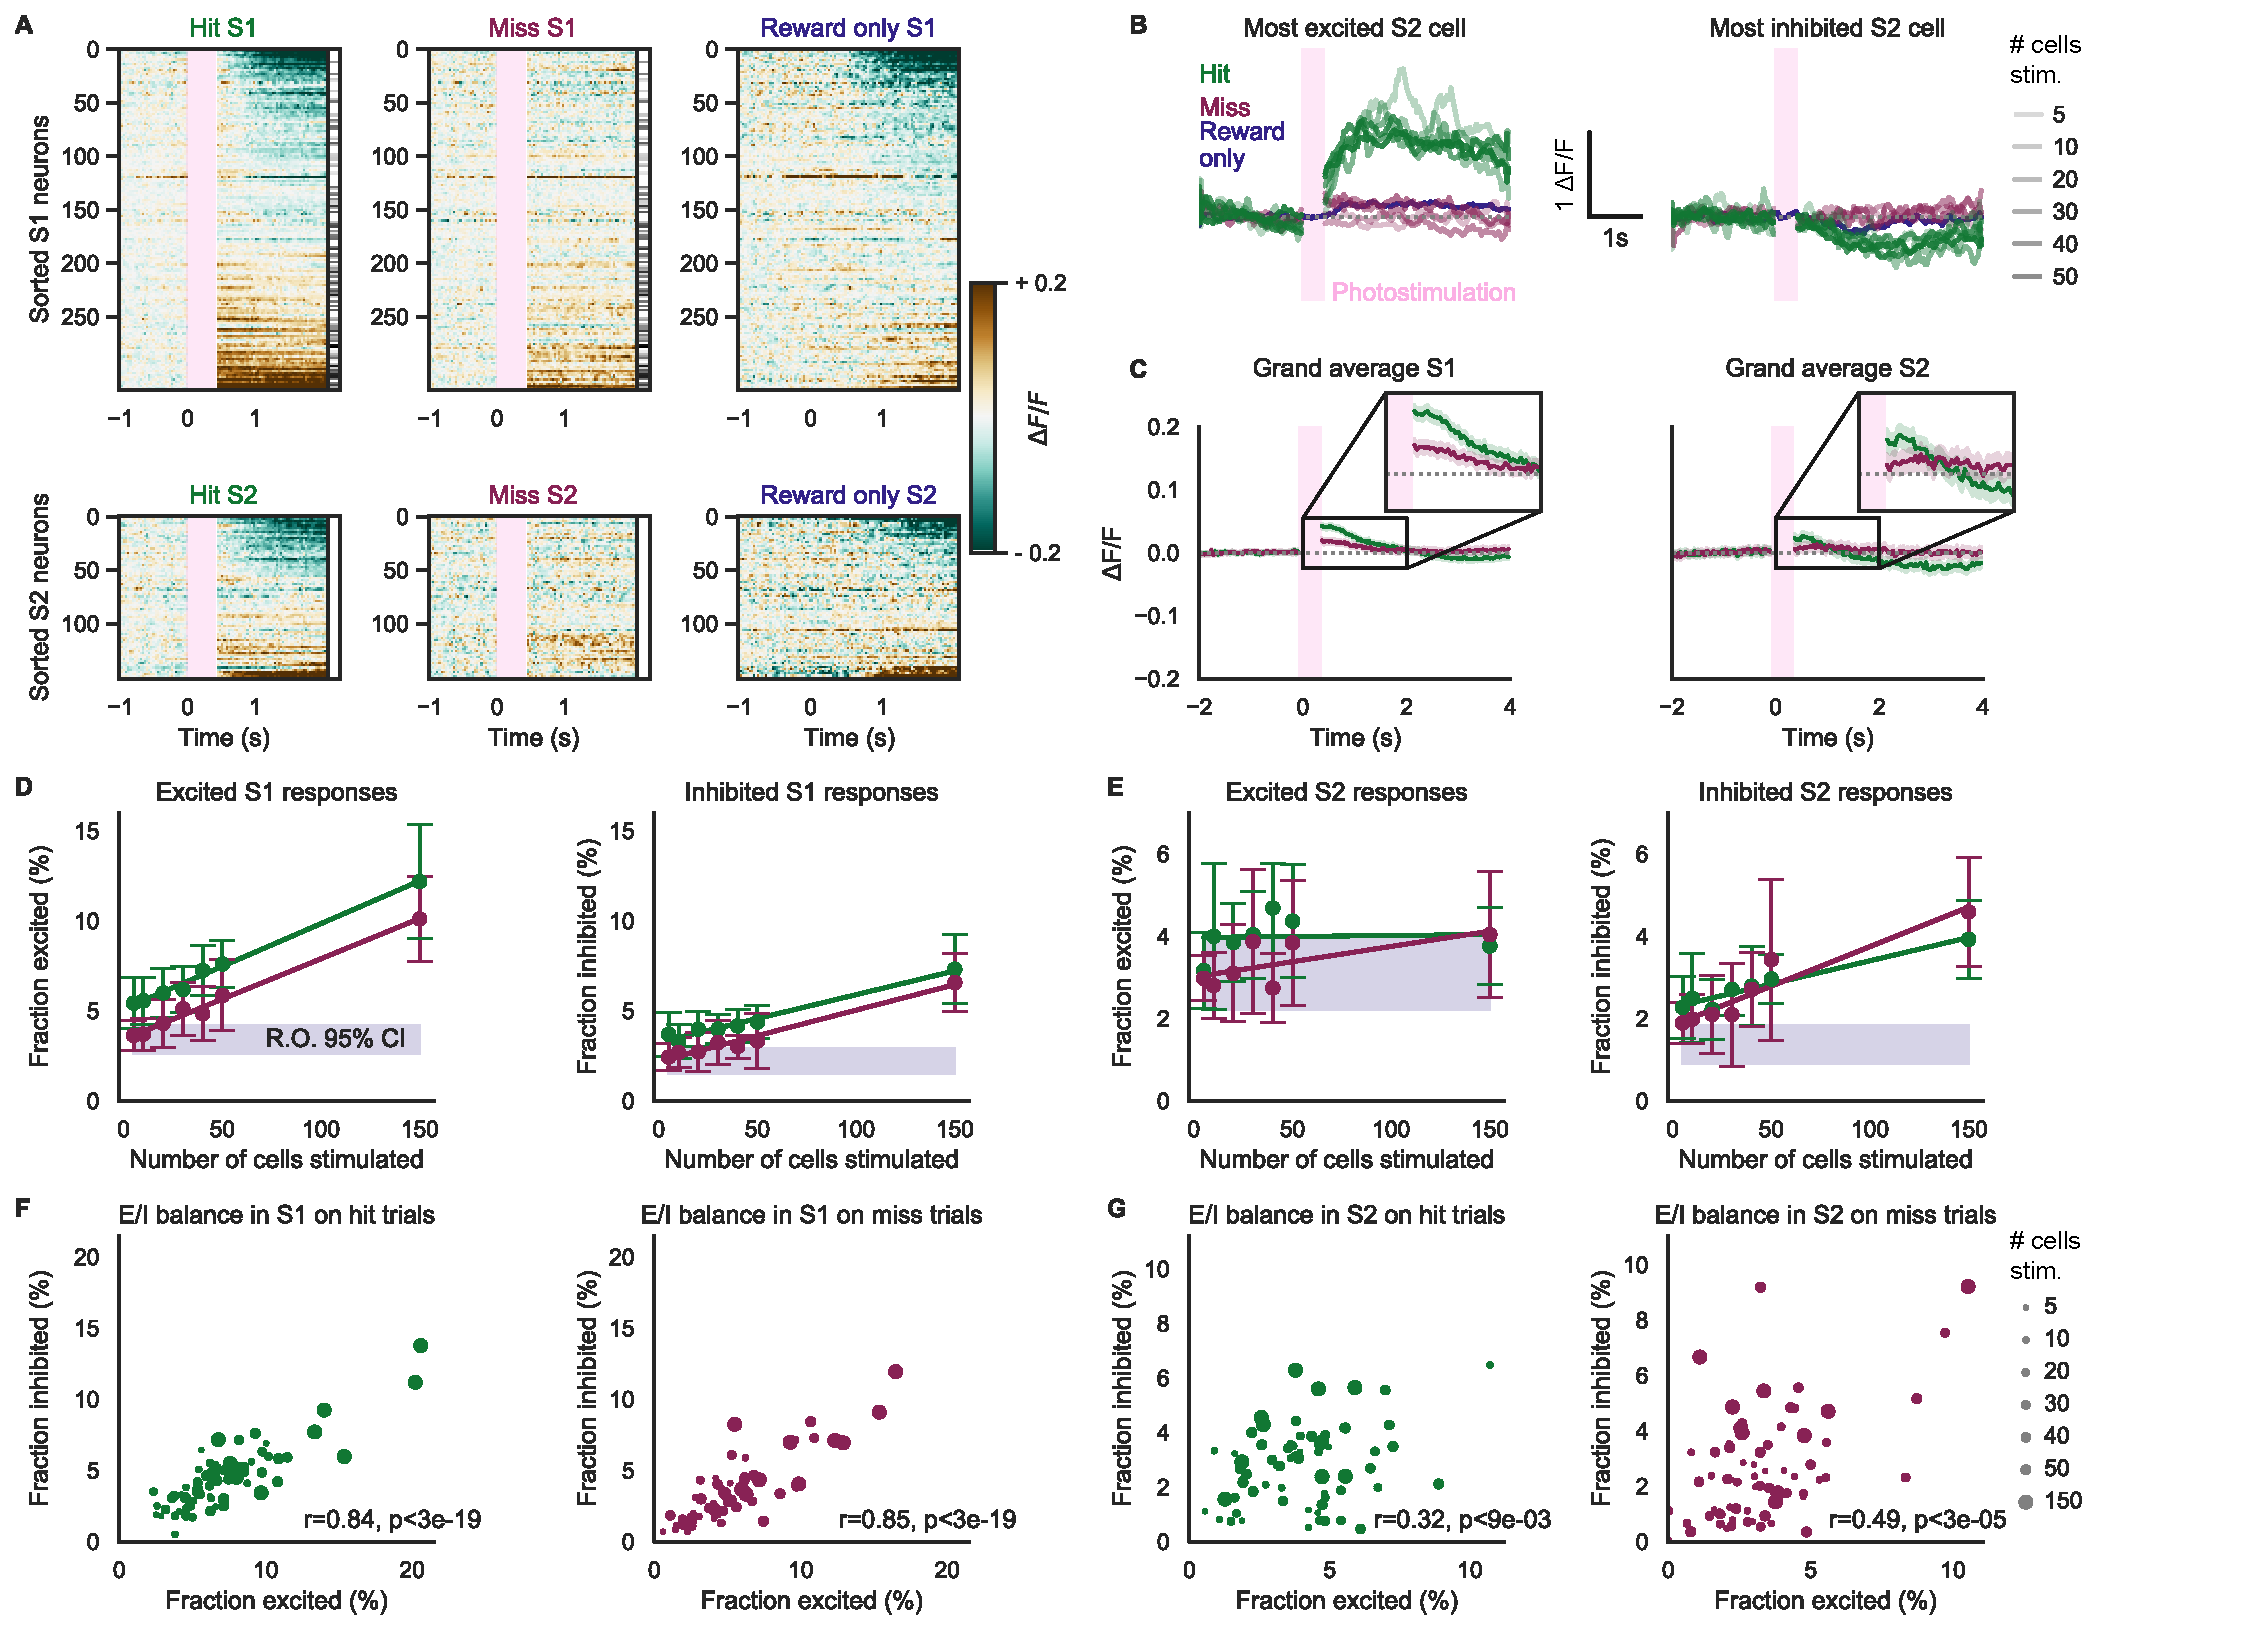
\includegraphics[scale=0.45]{figures/basic-analysis.pdf}
\caption[\textbf{Structure of evoked activity in S1 and S2}]{
\textbf{Structure of evoked activity in S1 and S2}. \textbf{(A)} Raster plots showing the trial averaged response to trial types (\textit{Left}: hit, \textit{Middle}: miss, \textit{Right}: reward only) to photostimulation (pink vertical bar, hit/miss)  and/or reward (hit/reward only) of individual cells from a single session. Data were baselined to the pre-stimulus mean on a cell-wise basis before averaging. Cells are sorted by the pairwise correlation between their trial averaged responses across all three trial types (methods). A clear excitatory and inhibitory response is elicited in S1 and S2 on hit trials that cannot be solely attributed to reward. The intensity of the bar on the right hand side of the hit and miss rasters is proportional to the number of times each cell was directly targeted by the photostimulation beam. Trials in which 150 cells were stimulated were removed for display. Data are blanked while the photostimulation laser was on (pink bar). \textbf{(B)} \textit{Left}: Example S2 cell excited on hit trials (green) but showing no response to miss trials (red) or reward only trials (blue). Each line shows an individual trial. The transparency of the line indicates the number of cells stimulated in S1. Individual trials were baselined to the pre-stimulus mean. \textit{Right}: Example S2 cell inhibited on hit trials. Trials in which 150 cells were stimulated were removed for display. \textbf{(C)} Average population response to hit and miss trials across all sessions. Traces are averaged across cells, trials and sessions for a given trial type. Individual trials were baselined to the pre-stimulus mean. Trials in which 150 cells were stimulated were removed for display. \textbf{(D)} Function mapping the response in S1 on hit and miss trials to the number of cells stimulated in S1. \textit{Left}: The fraction of excited cells in S1 maps linearly to the number of cells photostimulated on both hit and miss trials. \textit{Right}: The fraction of inhibited cells in S1 maps linearly to the number of cells photostimulated on both hit and miss trials. The shaded purple bar shows the fraction of excited or inhibited cells in S1 on reward only (R.O.) trials. \textbf{(E)} Function mapping the response in S2 on hit and miss trials to the number of cells stimulated in S1. \textit{Left}: There is no relationship between the fraction of excited cells in S2 and the number of cells stimulated in S1 on hit trials or miss trials. The shaded purple bar shows the fraction of excited or inhibited cells in S2 on reward only trials. \textit{Right}: The fraction of inhibited cells in S2 maps linearly to the number of cells photostimulated in S1 on both hit and miss trials. \textbf{(F)} Population E/I balance in S1 following photostimulation. The fraction of cells excited by photostimulation in S1 is highly correlated with the fraction of cells inhibited both on hit trials (\textit{left}) and miss trials (\textit{right}). The size of the circle indicates the number of cells photostimulated. \textbf{(G)} Population E/I balance in S2 following photostimulation in S1. The fraction of cells excited by photostimulation in S1 is significantly correlated with the fraction of cells inhibited both on hit trials (\textit{left}) and miss trials (\textit{right}). However the magnitude of the correlation is lower than in S1. The size of the circle indicates the number of cells photostimulated. 
} 
\label{fig:basic-analysis}
\end{figure}

Interestingly however, averaging responses across cells, trials and sessions reveals that hit trials elicit only a modest increase in population activity from baseline, immediately following stimulation, in S1 and S2, followed by a prolonged period of inhibition. Whereas the reward only condition exhibited a very different time course (Figure \ref{fig:supp1}B,C). This hints that both brain regions exist in balanced regimes whereby excitation driven by photostimulation results in inhibition of roughly equal magnitude. Miss trials elicit excitation following photostimulation in S1, however this excitation is not observed as propagated activity in trial-and-cell-averaged responses downstream in S2 (Figure \ref{fig:basic-analysis}C). 


\begin{figure}[h]
\hspace*{-0.25in}
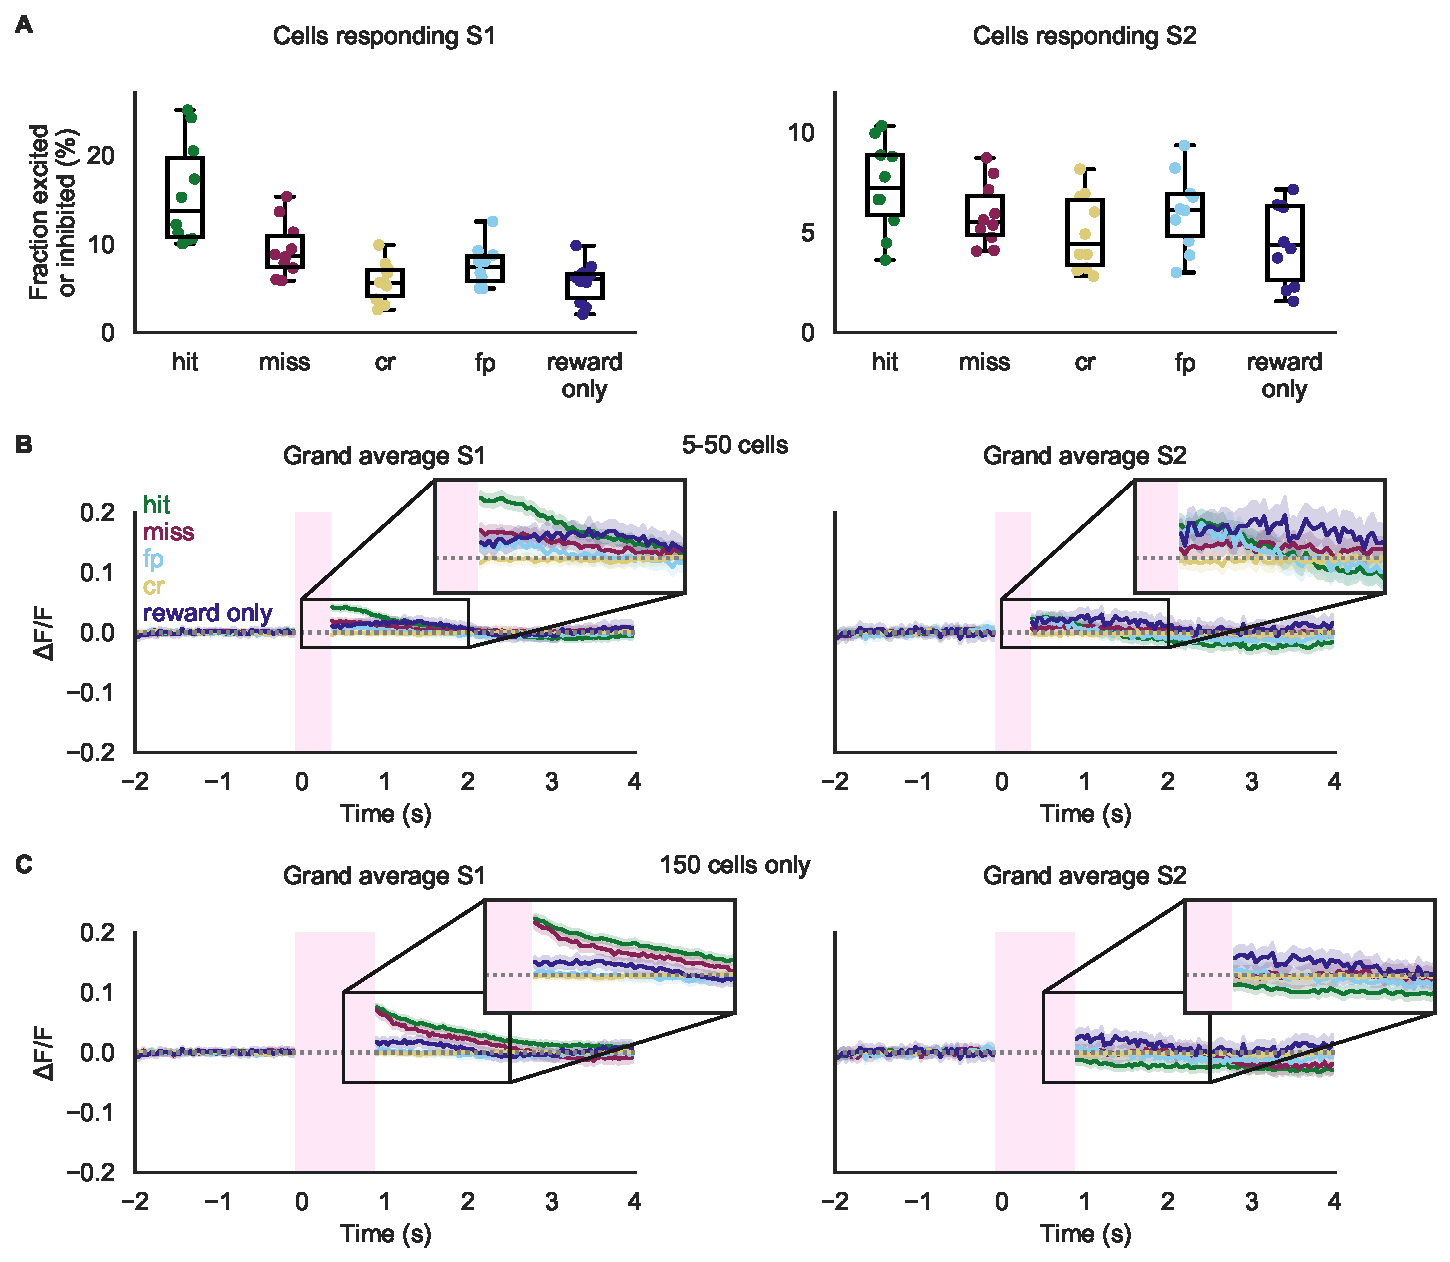
\includegraphics[scale=0.65]{figures/supplements/Supplementary_Figure1.pdf}
\caption[\textbf{Fraction of cells responding and grand average traces of all trial types in S1 and S2}]{\textbf{ Fraction of cells responding and grand average traces of all trial types in S1 and S2.
 (A)} The fraction of responsive cells (both excited and inhibited; methods) on each trial type across all numbers of cells stimulated. \textbf{(B)} Average population response to all trial types across all sessions. Traces are averaged across cells, trials and sessions for a given trial type. Individual trials were baselined to the pre-stimulus mean. Trials in which 150 cells were stimulated were removed for display. \textbf{(C)} As above but including only trials in which 150 cells were stimulated. 
} 
\label{fig:supp1}
\end{figure}


We next compared how the percentage of excited or inhibited neurons, both locally in S1 and downstream in S2, scaled with the number of cells photostimulated in S1 and whether this differed between perceived and non-perceived stimuli (Figure \ref{fig:basic-analysis}D,E). As expected, stimulating more neurons in S1 excited a greater percentage of the population regardless of whether the stimulus was perceived (Figure \ref{fig:basic-analysis}D left)  (Pearson’s r = 0.62, p  = 1.8x10\textsuperscript{-8} hit trials; Pearson’s r = 0.65, p = 2.4x10\textsuperscript{-9} miss trials). We also find that the percentage of inhibited cells in S1 also scales linearly with the number of cells stimulated (Figure \ref{fig:basic-analysis}D right) (Pearson’s r = 0.55, p = 1.2x10\textsuperscript{-6} hit trials; Pearson’s r = 0.59, p = 1.4x10\textsuperscript{-7} miss trials). This indicates that excitatory photostimulation elicits a compensatory inhibitory response local to the stimulation. In S2, downstream of the stimulation, however the population response to increasing numbers of stimulated cells is more complex. We find no significant relationship between the percentage of excited cells in S2 and the number of stimulated cells in S1 on hit trials or miss trials, although the correlation is an order of magnitude greater on miss trials (Pearson’s r = 0.01, p = 0.9 hit trials; Pearson’s r = 0.17, p = 0.16 miss trials). However we find that the percentage of inhibited cells in S2 scales linearly with the number of stimulated cells in S1 both on hit and on miss trials (Figure \ref{fig:basic-analysis}E left, right) (Pearson’s r = 0.37, p = 0.002 hit trials; Pearson’s r = 0.45, p = 1.2x10\textsuperscript{-4} miss trials).

Next, we explicitly quantified the balance between excitation and inhibition (E/I) in both brain regions. We find robustly maintained E/I balance in S1 regardless of whether or not the stimulation was perceived, whereby the percentage of cells excited and inhibited is highly correlated (Figure \ref{fig:basic-analysis}F) (Pearson’s r = 0.84, p < 3x10\textsuperscript{-19} hit trials; Pearson’s r = 0.85, p < 3x10\textsuperscript{-19} miss trials). Downstream in S2, we also find E/I balance both on hit trials and miss trials, however the correlation is less strong than in S1, and is weaker on hit trials than miss trials (Figure \ref{fig:basic-analysis}G) (Pearson’s r = 0.32, p < 0.009 hit trials; Pearson’s r = 0.49, p < 3x10\textsuperscript{-5} miss trials). Taken together, we show that as activity is propagated away from its site of initiation, E/I balance persists but its strength is reduced. Additionally, perceived stimuli escape the balanced regime downstream to a greater extent than non-perceived stimuli as evidenced by the stronger correlation between the percentage of excited and inhibited cells on miss trials compared to hit trials. 


\begin{figure}[h]
\hspace*{-0.6in}
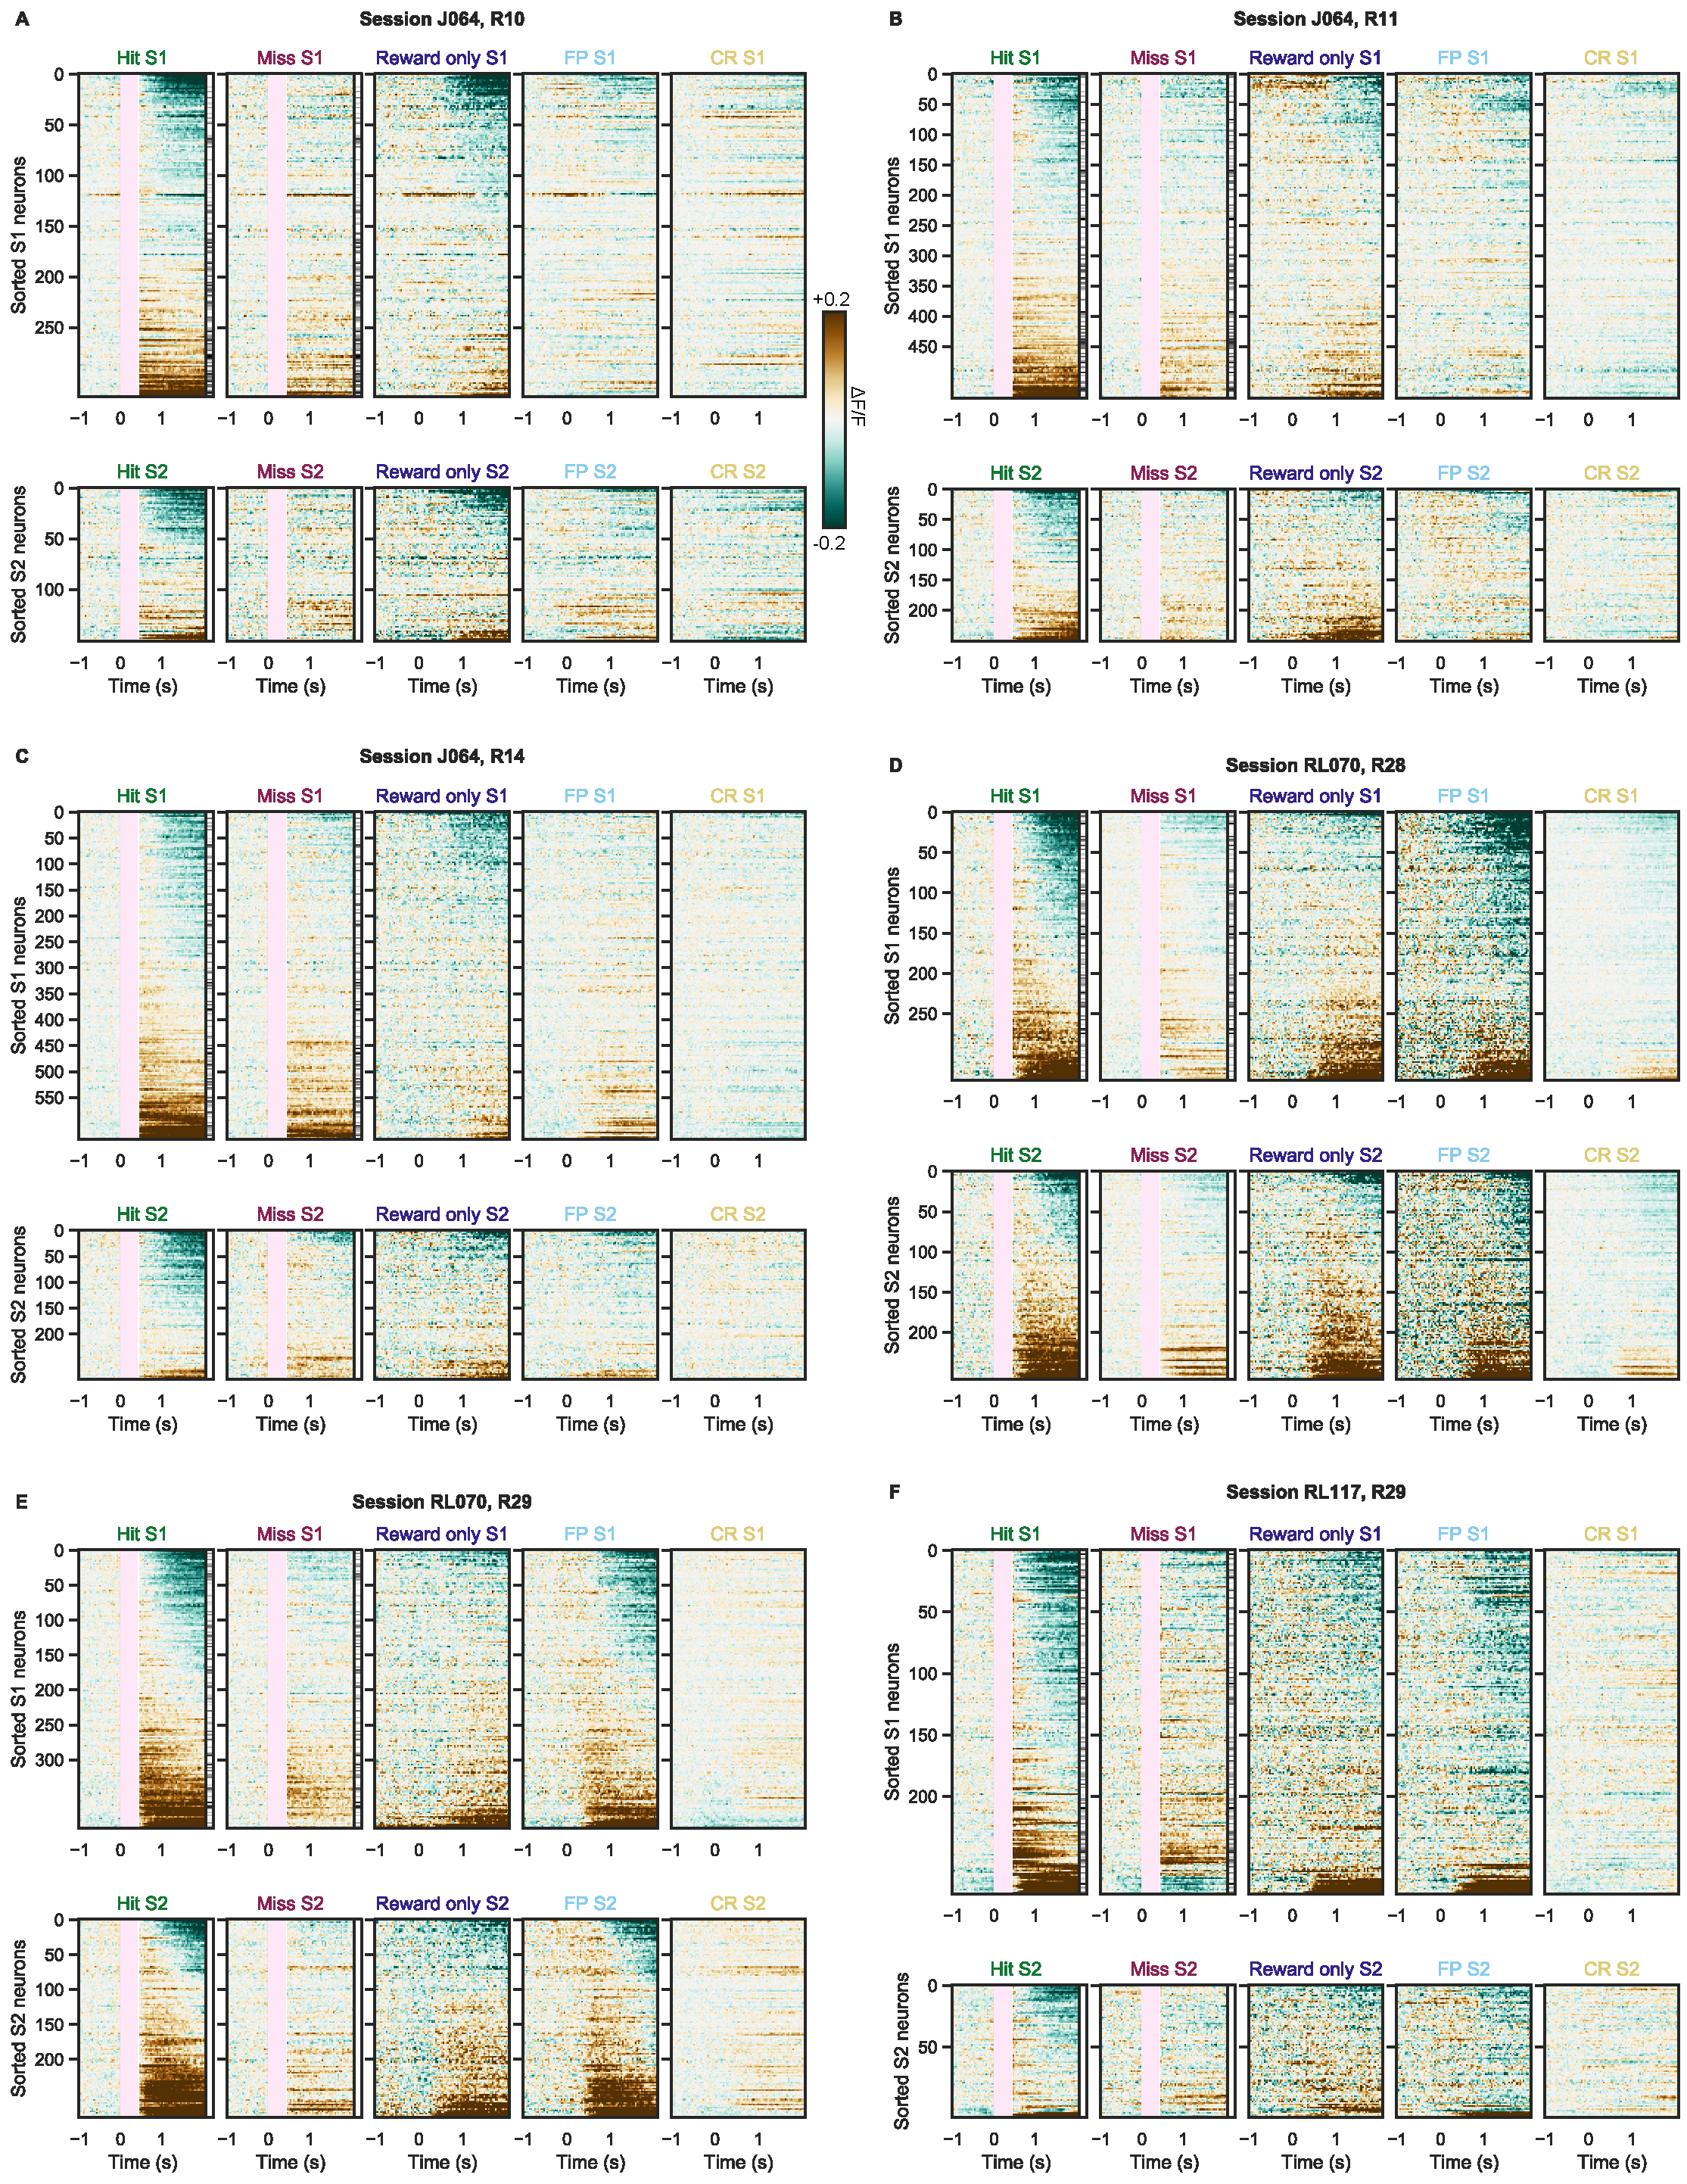
\includegraphics[scale=0.45]{figures/supplements/Supplementary_Figure2.pdf}
\caption[\textbf{Trial averaged raster plots for all sessions and trial types}]{\textbf{Trial averaged raster plots for all sessions and trial types}
\textbf{(A-F)} Raster plots showing the trial averaged response to trial types to photostimulation (pink vertical bar, hit/miss) and/or reward (hit/reward only) and/or licks (hit/reward only/false positive) of individual cells from 6 sessions. Data were baselined to the pre-stimulus mean on a cell-wise basis before averaging. Cells are sorted by the pairwise correlation between their trial averaged responses across all three trial types.
} 
\label{fig:supp2}
\end{figure}

\begin{figure}[h]
\hspace*{-0.6in}
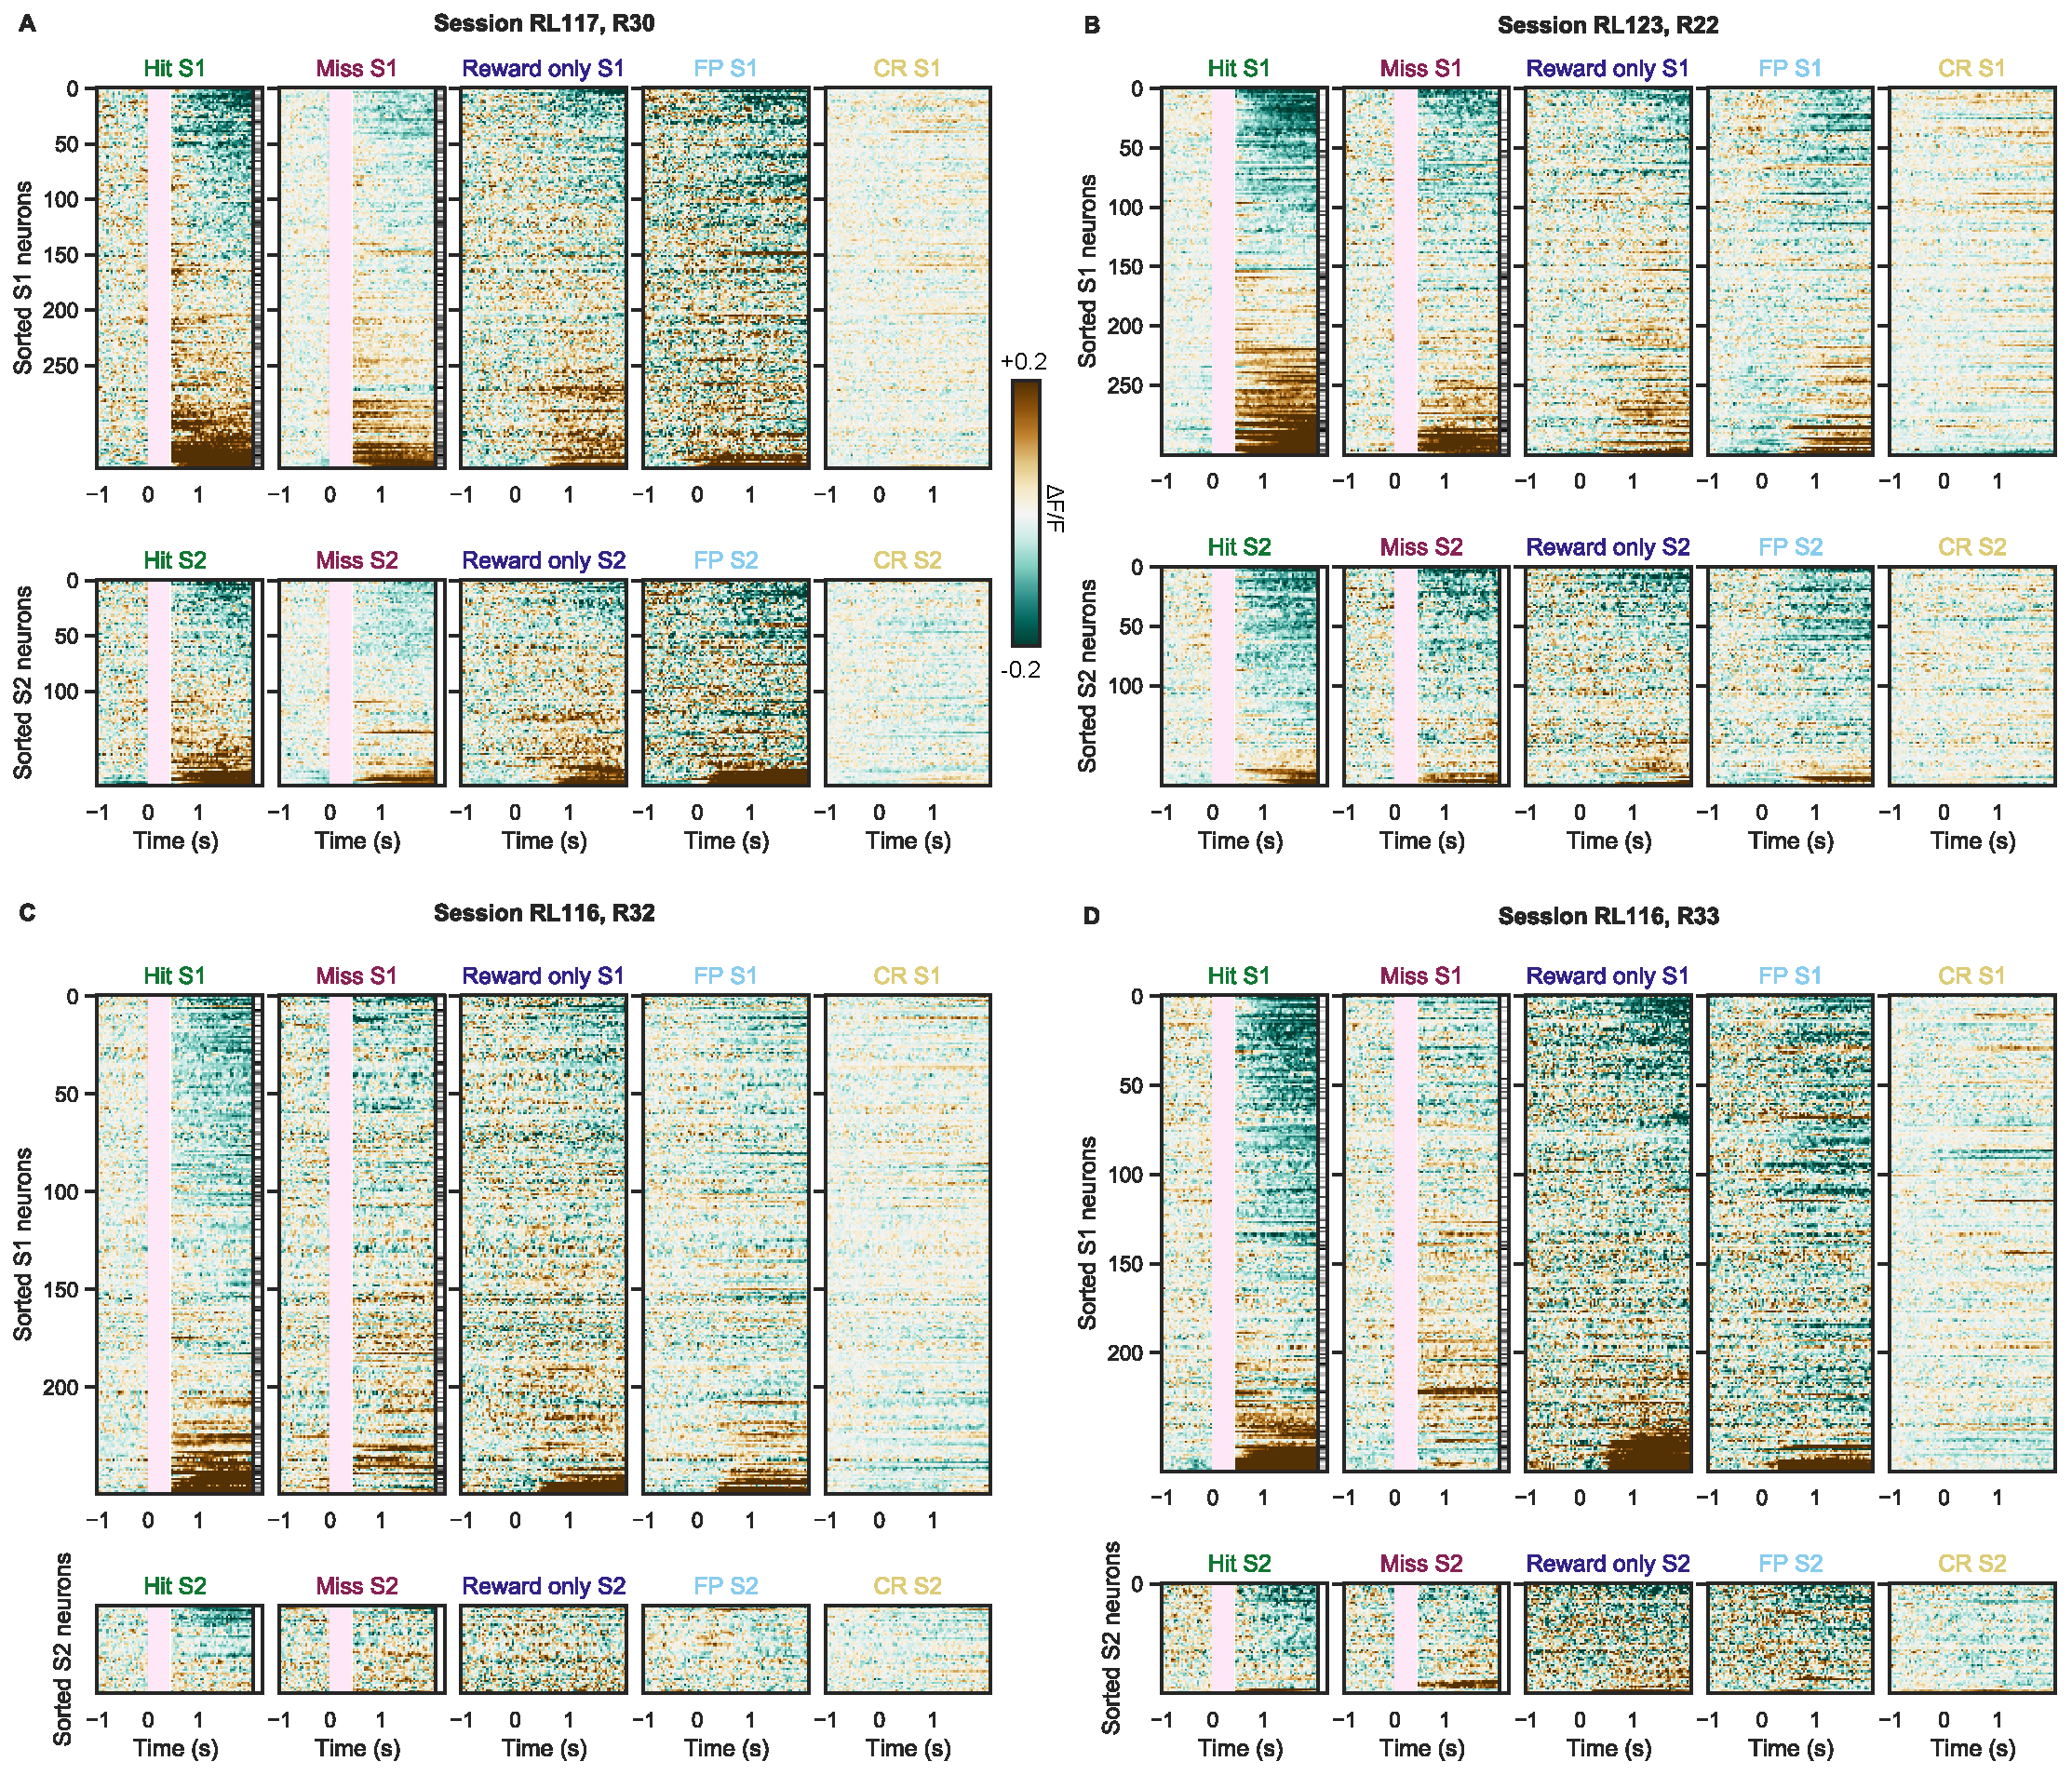
\includegraphics[scale=0.45]{figures/supplements/Supplementary_Figure3.pdf}
\caption[\textbf{Trial averaged raster plots for all sessions and trial types: continued}]{\textbf{Trial averaged raster plots for all sessions and trial types: continued}
\textbf{(A-D)} As above for the remaining 4 sessions
} 
\label{fig:supp3}
\end{figure}

\section{Perceived photostimulation elicit persistent activity in both S1 and S2 populations}

As shown in the previous section, individual cells display a diverse array of responses, and balanced mean average responses mask the magnitude and time course of propagated activity (Figure \ref{fig:basic-analysis}). To gain insight into these complex neural responses, we employed logistic regression classifiers on the network level and assessed propagation of stimulus-relevant activity and its relationship to behaviour. We trained classifiers to decode the trial type of individual trials using the activity of all cells in S1 or S2 on imaging data from single imaging frames. This allowed us to uncover the neural signatures of each trial type in both brain regions and quantify the temporal dynamics of this signature. First, we trained a model to classify hit trials from correct rejection trials, meaning the model should detect the neural signature of both the stimulus and the activity resulting in its perception. The classifier performed significantly above chance after stimulation and performance remained well above chance for several seconds both in S1 and S2 (two-sided Wilcoxon signed-rank test, p < 0.05, Bonferroni corrected) (Figure \ref{fig:fig3}A left, B left; Figure \ref{fig:supp4}A,B,G,H; Figure \ref{fig:supp5}A left, B left). Therefore, the neural activity underpinning perceived stimulation persisted both locally in S1 and downstream in S2 for several seconds. However, the classifier could be decoding the signatures of reward and the motor command required for licking, which are present on hit trials but not correct rejection trials. To address this, we tested the pre-trained classifier on reward only trials in which reward was delivered in the absence of photostimulation. In S1, performance on this trial type was either below or at chance level (p < 0.05, Bonferroni corrected); in S2, classifier performance on reward only trials remained at chance throughout the first 2.7 seconds of the trial (Figure \ref{fig:fig3}A left, B left; Figure \ref{fig:supp4}A,B,G,H; Figure \ref{fig:supp5}A left, B left) (p < 0.05, Bonferroni corrected). 


\begin{figure}[!h]
\hspace*{-0.2in}
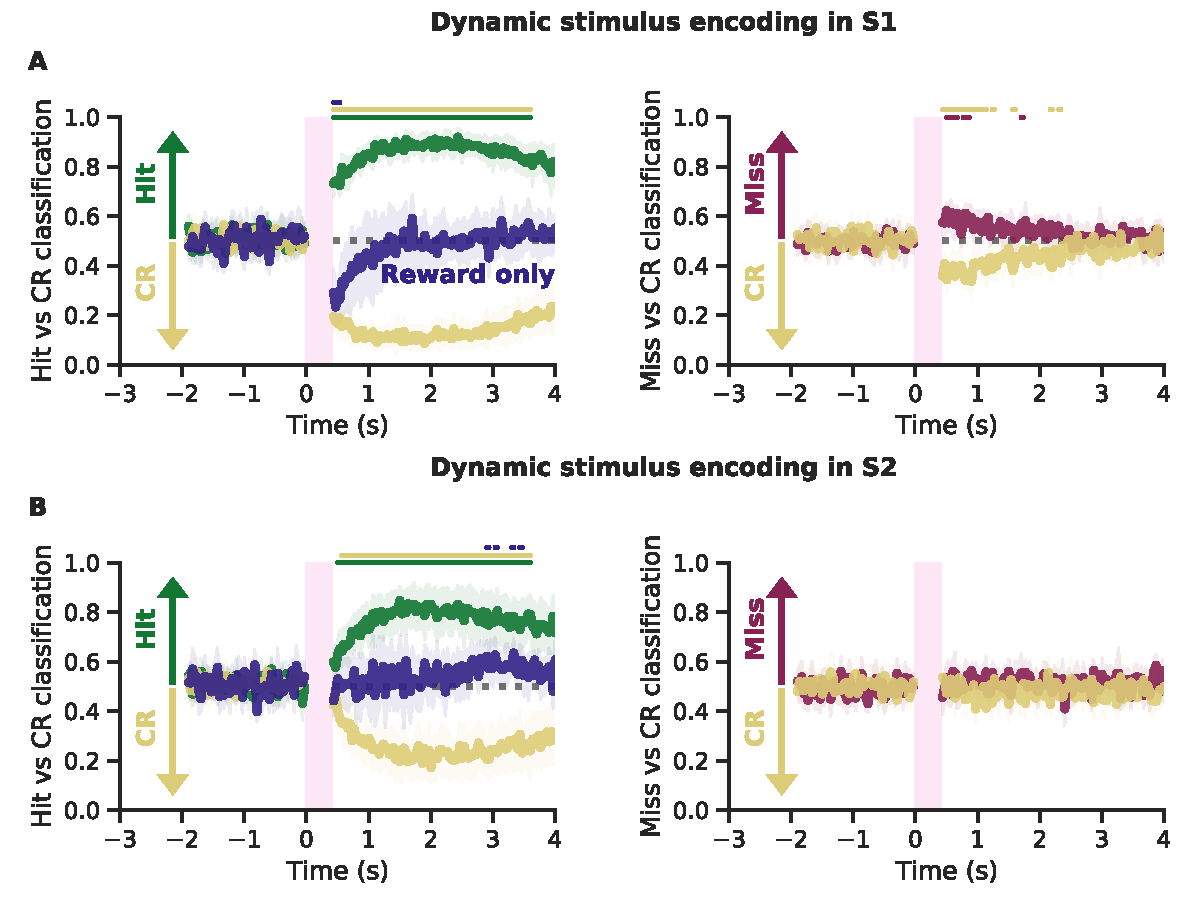
\includegraphics[scale=0.76]{figures/Figure3.pdf}
\caption[\textbf{Perceived photostimuli elicit persistent activity in both S1 and S2 populations.
}]{\textbf{Perceived photostimuli elicit persistent activity in both S1 and S2 populations} Dynamic decoding of trial type from neural activity in S1 using a logistic regression model. Models were trained on each frame individually, with activity from every cell in S1 or S2, and tested on held out data. Coloured bars above the traces show timepoints at which classifier performance was significantly different from chance (see methods).
\textbf{(A)} \textit{Left}: A model was trained on S1 activity to classify hit trials from correct rejection trials and then tested on hit trials (green), correct rejection trials (yellow) and reward only trials (blue). The model is able to classify hit trials from correct rejection trials for several seconds following photostimulation, implying that activity arising from perceived stimulation persists in S1. Reward only trials were not classified as hits, showing that the model was not just trained to decode the neural signature of reward on hit trials. \textit{Right}: A model was trained on S1 activity to classify miss trials from correct rejection trials and then tested on miss trials (red) and correct rejection trials (yellow). The model is able to distinguish the two trial types for only for ~1 second following stimulation. This implies that non-perceived stimuli do not generate persistent activity. \textbf{(B)} \textit{Left}: A model was trained on S2 activity to classify hit trials from correct rejection trials and then tested on hit trials (green), correct rejection trials (yellow) and reward only trials (blue). As above, the model is able to classify hit trials from correct rejection trials for several seconds following photostimulation, implying that activity arising from perceived stimulation in S1 is propagated to S2 and persists for several seconds. Reward only trials were not classified as hits, indicating that the model was not just detecting the neural signature of reward on hit trials. \textit{Right}: A model was trained on S2 activity to classify miss trials from correct rejection trials and then tested on miss trials (red) and correct rejection trials (yellow). The model was not able to classify miss from correct rejection trials at any timepoint, indicating that non-perceived stimuli were not robustly propagated from S1 to S2.
} 
\label{fig:fig3}
\end{figure}

\begin{figure}[!h]
\hspace*{-0.2in}
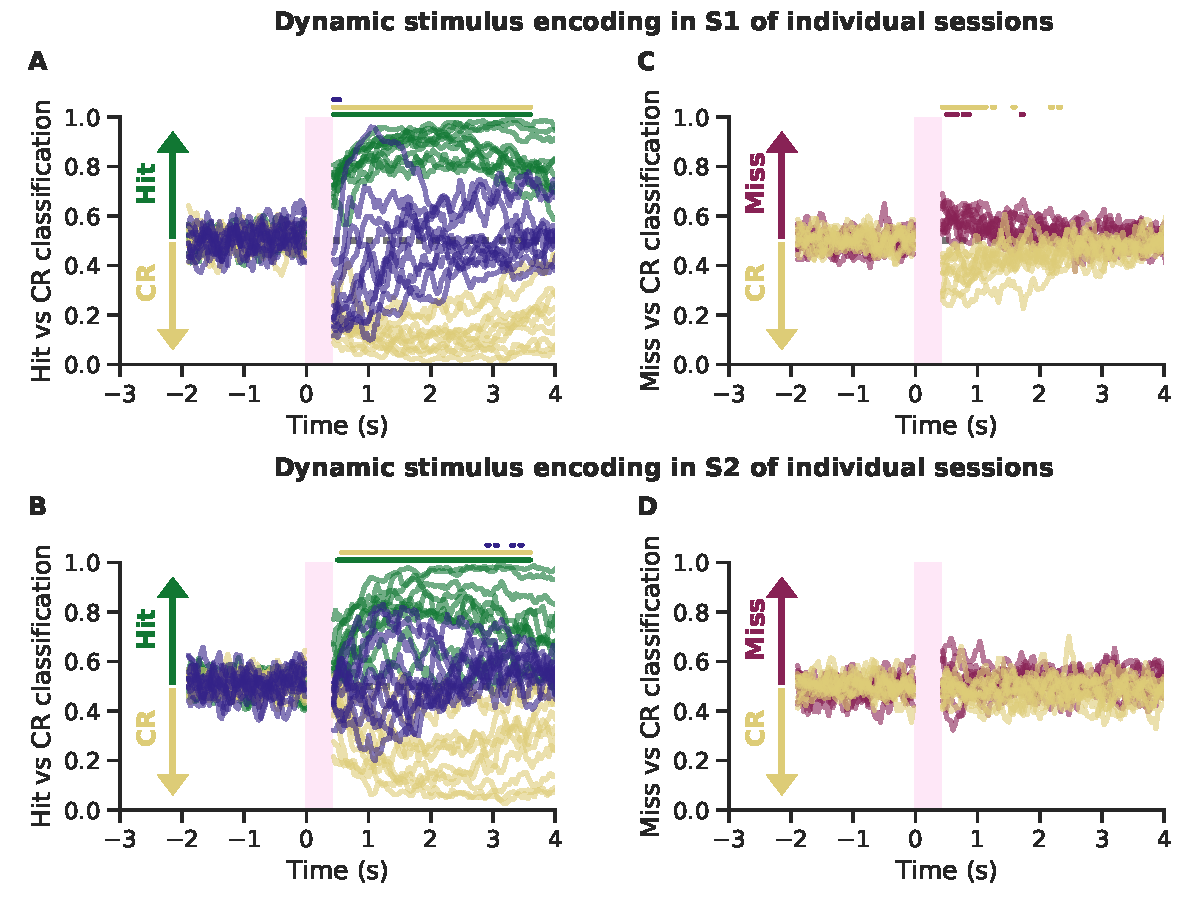
\includegraphics[scale=0.76]{figures/supplements/Supplementary_Figure5.pdf}
\caption[\textbf{Dynamic decoders of individual sessions}]{\textbf{Dynamic decoders of individual sessions} As figure \ref{fig:fig3}, but displaying classifier performance for each individual sessions. Individual sessions are shown as more transparent lines, with the session average as a fully opaque line.
} 
\label{fig:supp5}
\end{figure}

As reward signals in the brain are complex, and depend on whether the reward is expected or unexpected \cite{schultz_multiple_2000}, we confirmed that the reward signal on hit trials and reward only trials was comparable, thus ensuring that the hit vs correct rejection classifier was indeed classifying the neural signature of perceived stimulation and not just reward. This is critical as the water reward on hit trials was expected, but not expected on reward only trials. We addressed this by training a model to classify reward only trials from correct rejection trials, thus this classifier should detect only the neural signal from rewards (Figure \ref{fig:supp4}E,F). Testing this model on hit trials resulted in identical performance to the reward only condition both in S1 and S2 (no significant difference on 110/110 time points in S1 and 108/110 time points in S2). This means that a classifier trained specifically to detect rewards could not distinguish hit and reward only trials, meaning that the neural response to reward is comparable in both trial types and the classification of hit trials from correct rejection trials is indeed decoding the neural signature of perceived stimulation, both in S1 and S2.


\begin{figure}[h]
\vspace*{-3cm}
\thisfloatpagestyle{empty}
% \hspace*{-0.2in}
\vspace*{-0.2cm}
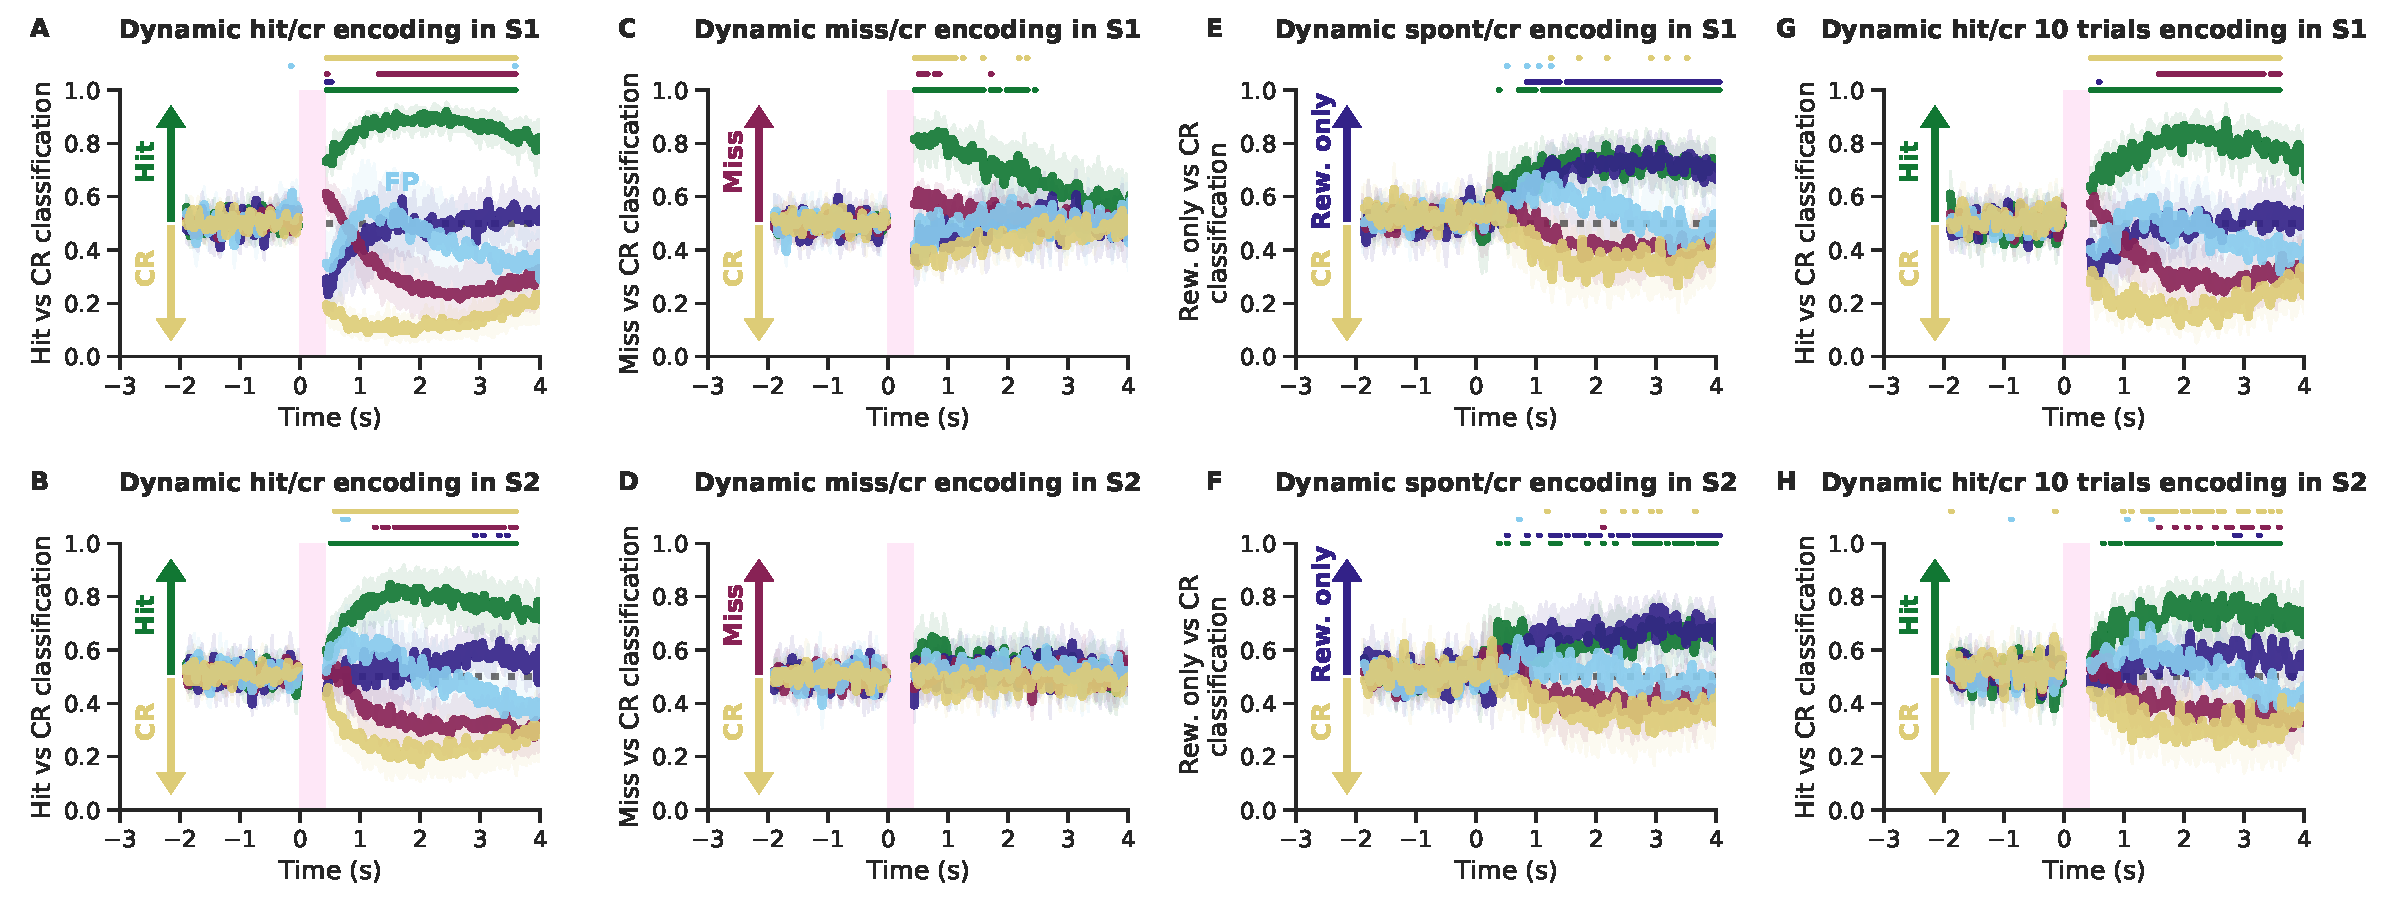
\includegraphics[scale=0.7]{figures/supplements/Supplementary_Figure4.pdf}
\caption[\textbf{Dynamic decoders of all trial types}]{\textbf{Dynamic decoders of all trial types} 

Dynamic decoding of trial type from neural activity in S1 using a logistic regression model. Models were trained on each frame individually, with activity from every cell in S1 or S2, and tested on held out data. Coloured bars above the traces show timepoints at which classifier performance was significantly different from chance (see methods). \textbf{(A)} A model was trained on S1 activity to classify hit trials from correct rejection trials and then tested on hit trials (green), correct rejection trials (yellow), reward only trials (dark blue), false positive trials (light blue) and miss trials (red). \textbf{(B)} As above, but trained on S2 activity. \textbf{(C)} A model was trained on S1 activity to classify miss trials from correct rejection trials and then tested on miss trials (red), correct rejection trials (yellow) reward only trials (dark blue), false positive trials (light blue) and hit trials (green). \textbf{(D)} As above, but trained on S2 activity. \textbf{(E)} A model was trained on S1 activity to classify reward only trials from correct rejection trials and then tested on reward only (dark blue), correct rejection trials (yellow), miss trials (red), false positive trials (light blue) and hit trials (green).\textbf{(F)} As above, but trained on S2 activity. \textbf{(G)} As \textbf{(A)} but the number of trials was restricted to 10 for each type, matching the total number of reward only trials recorded. \textbf{(H)} As \textbf{(B)} but the number of trials was restricted to 10 for each type, matching the total number of reward only trials recorded.
} 
\label{fig:supp4}
\end{figure}

Next we asked whether non-perceived neural activity was reliably propagated from S1 to S2 by training a model to classify miss and correct rejection trials (Figure \ref{fig:fig3}A right, B right; Figure \ref{fig:supp4}C,D; Figure \ref{fig:supp5}A right B right).

We found that in S1, this model decoded miss trials slightly above chance immediately following stimulation (p < 0.05, Bonferroni corrected), however performance rapidly decayed back to chance level after ~1 second. Conversely in S2, the model did not perform above chance at any point in time, indicating that stimulus information that is not perceived does not propagate to S2.

Taken together, these results show that only perceived stimulus representations are reliably propagated out of the local brain region in which they originate to a downstream brain area. Further, stimuli that are propagated and drive perception persist both locally and downstream for several seconds following the initial injection of activity.

\section{Pre-stimulus population in S1 predicts the upcoming trial outcome}

To address the conditions facilitating both the propagation of activity to S2 and the behavioural response to stimulus, we measured population activity in S1 immediately prior to stimulation (Figure \ref{fig:figure4}A) and asked whether any statistic of the pre-stimulus population activity could predict whether the stimulus would be perceived (i.e. whether the upcoming trial type would be a hit or a miss) (see methods). This allows us to assess how population activity is formatted pre-stimulus to gate whether the upcoming stimulation propagates and thus drives perception. One basic measure of population activity is the mean, measuring whether raised or suppressed activity across S1 prior to the stimulus arriving is predictive of an upcoming hit or miss trial. We find no evidence that this metric pre-stimulus is predictive of trial type (Figure \ref{fig:figure4}B left) (n.s.). Likewise, we find no evidence that the mean pairwise correlation between all pairs of neurons (methods) in S1 pre-stimulus increases or decreases the likelihood of stimulus detection (Figure \ref{fig:figure4}B center) (n.s.).


\begin{figure}[h!]
\vspace*{-1.5cm}
\thisfloatpagestyle{empty}
\hspace*{-0.4in}
% \vspace*{-0cm}
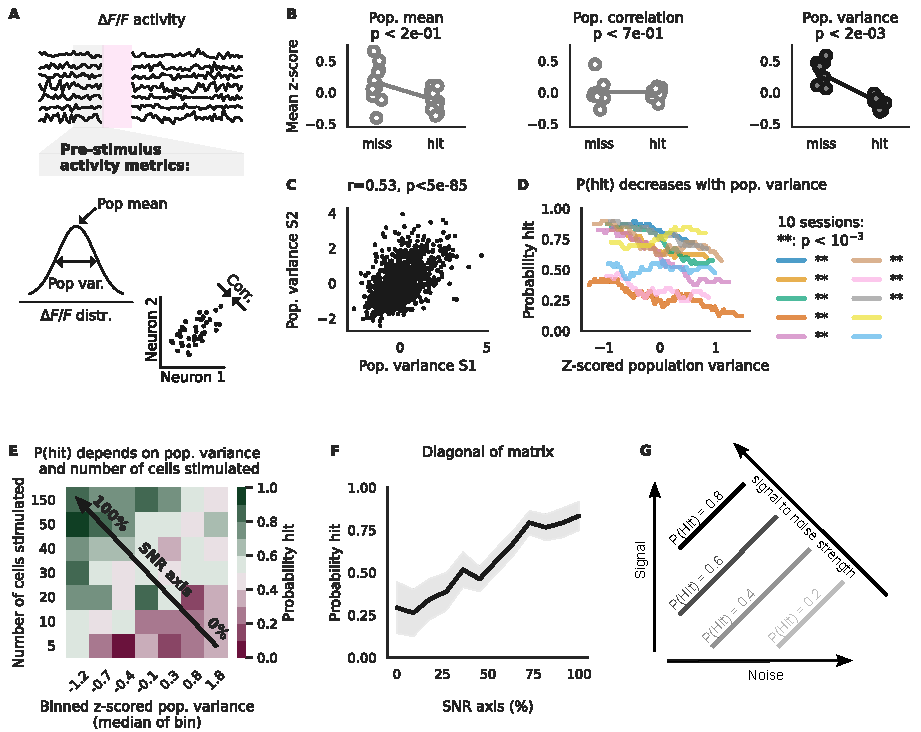
\includegraphics[scale=1.08]{figures/Figure4.pdf}
\caption[\textbf{Pre-stimulus population in S1 predicts the upcoming trial outcome}]{\textbf{Pre-stimulus population in S1 predicts the upcoming trial outcome} 

\textbf{(A)} Illustration of neural activity throughout a trial. Only the activity before the stimulus on a given trial is included in subsequent plots. We considered 3 metrics of pre-stimulus neural activity; the population mean, population variance and the average absolute correlation coefficient. \textbf{(B)} Comparison of population metrics of pre-stimulus S1 activity prior to hit trials and prior to miss trials. \textit{Left}: No evidence that mean population activity pre-stimulus predicts the upcoming trial outcome. \textit{Center}: No evidence that pre-stimulus pairwise Pearson correlation, averaged across all pairs of neurons, predicts upcoming trial outcome. \textit{Right}: Population variance is significantly higher before miss trials than before hit trials. Pre-stimulus population metrics in S1 were computed trial-wise and z-scored across trials within a session before being split into hit and miss trials and averaged across a session. P values tested for a difference in session-wise population metrics between hit and miss trials. \textbf{(C)} Population variance is significantly correlated between S1 and S2 on a single-trial level. \textbf{(D)} The probability of a hit trial as a function of pre-stimulus population variance in S1 on a single session level. Trials within a session were binned by their z-scored population variance and this was correlated to the probability of a hit trial within that bin. 8/10 sessions show a significant negative correlation between pre-stimulus population variance and the probability of a hit. \textbf{(E)} The interaction between pre-stimulus population variance in S1 and the number of cells photostimulated defines the probability of a hit trial. Trials within a session were binned by their z-scored population variance and by the number of cells photostimulated; the probability of a hit within each bin was plotted on a 2-dimensional axis. This was repeated for all sessions. Maximising the number of cells stimulated and minimising the pre-stimulus variance yielded the greatest probability of a hit trial. \textbf{(F)} Maximising the SNR of the stimulus resulted in the maximal probability of a hit trial. Data as in E, but projected onto the ‘SNR’ axis by averaging across all bins that project orthogonally onto each point on the axis. \textbf{(G)} Schematic outlining the intuition for the SNR axis. Increasing the number of cells stimulated on a given trial maximises the signal of that stimulus. Noise is inversely proportional to the population variance as there is more excitation and suppression from baseline in a population with high variance. The probability of hit is maximal when SNR is maximal as the stimulus is more likely to be detected above ongoing activity. 
} 
\label{fig:figure4}
\end{figure}

One metric that clearly predicts whether the upcoming stimulus will be propagated out of S1 to drive a hit is the population variance  (Figure \ref{fig:figure4}B right), defined as the variance of the distribution of activity across S1 neurons (methods). The lower the variance of the activity distribution pre-stimulus, the more likely the upcoming trial will be a hit. Prior to a miss trial, the variance of activity across neurons is greater than prior to a hit trial (p < 0.002). See Figure \ref{fig:supp6} for the further quantification of significant activity metrics of both S1 and S2.  Additionally, population variance in S1 is correlated to population variance in S2, (Figure \ref{fig:figure4}C) (Pearson’s r = 0.53, p < 5x10\textsuperscript{-85}) demonstrating that this phenomenon is not just limited to the directly photostimulated brain region and therefore may be a metric of a more global brain state.


\begin{figure}[h!]
\vspace*{-1.5cm}
\thisfloatpagestyle{empty}
\hspace*{-0.6in}
% \vspace*{-0cm}
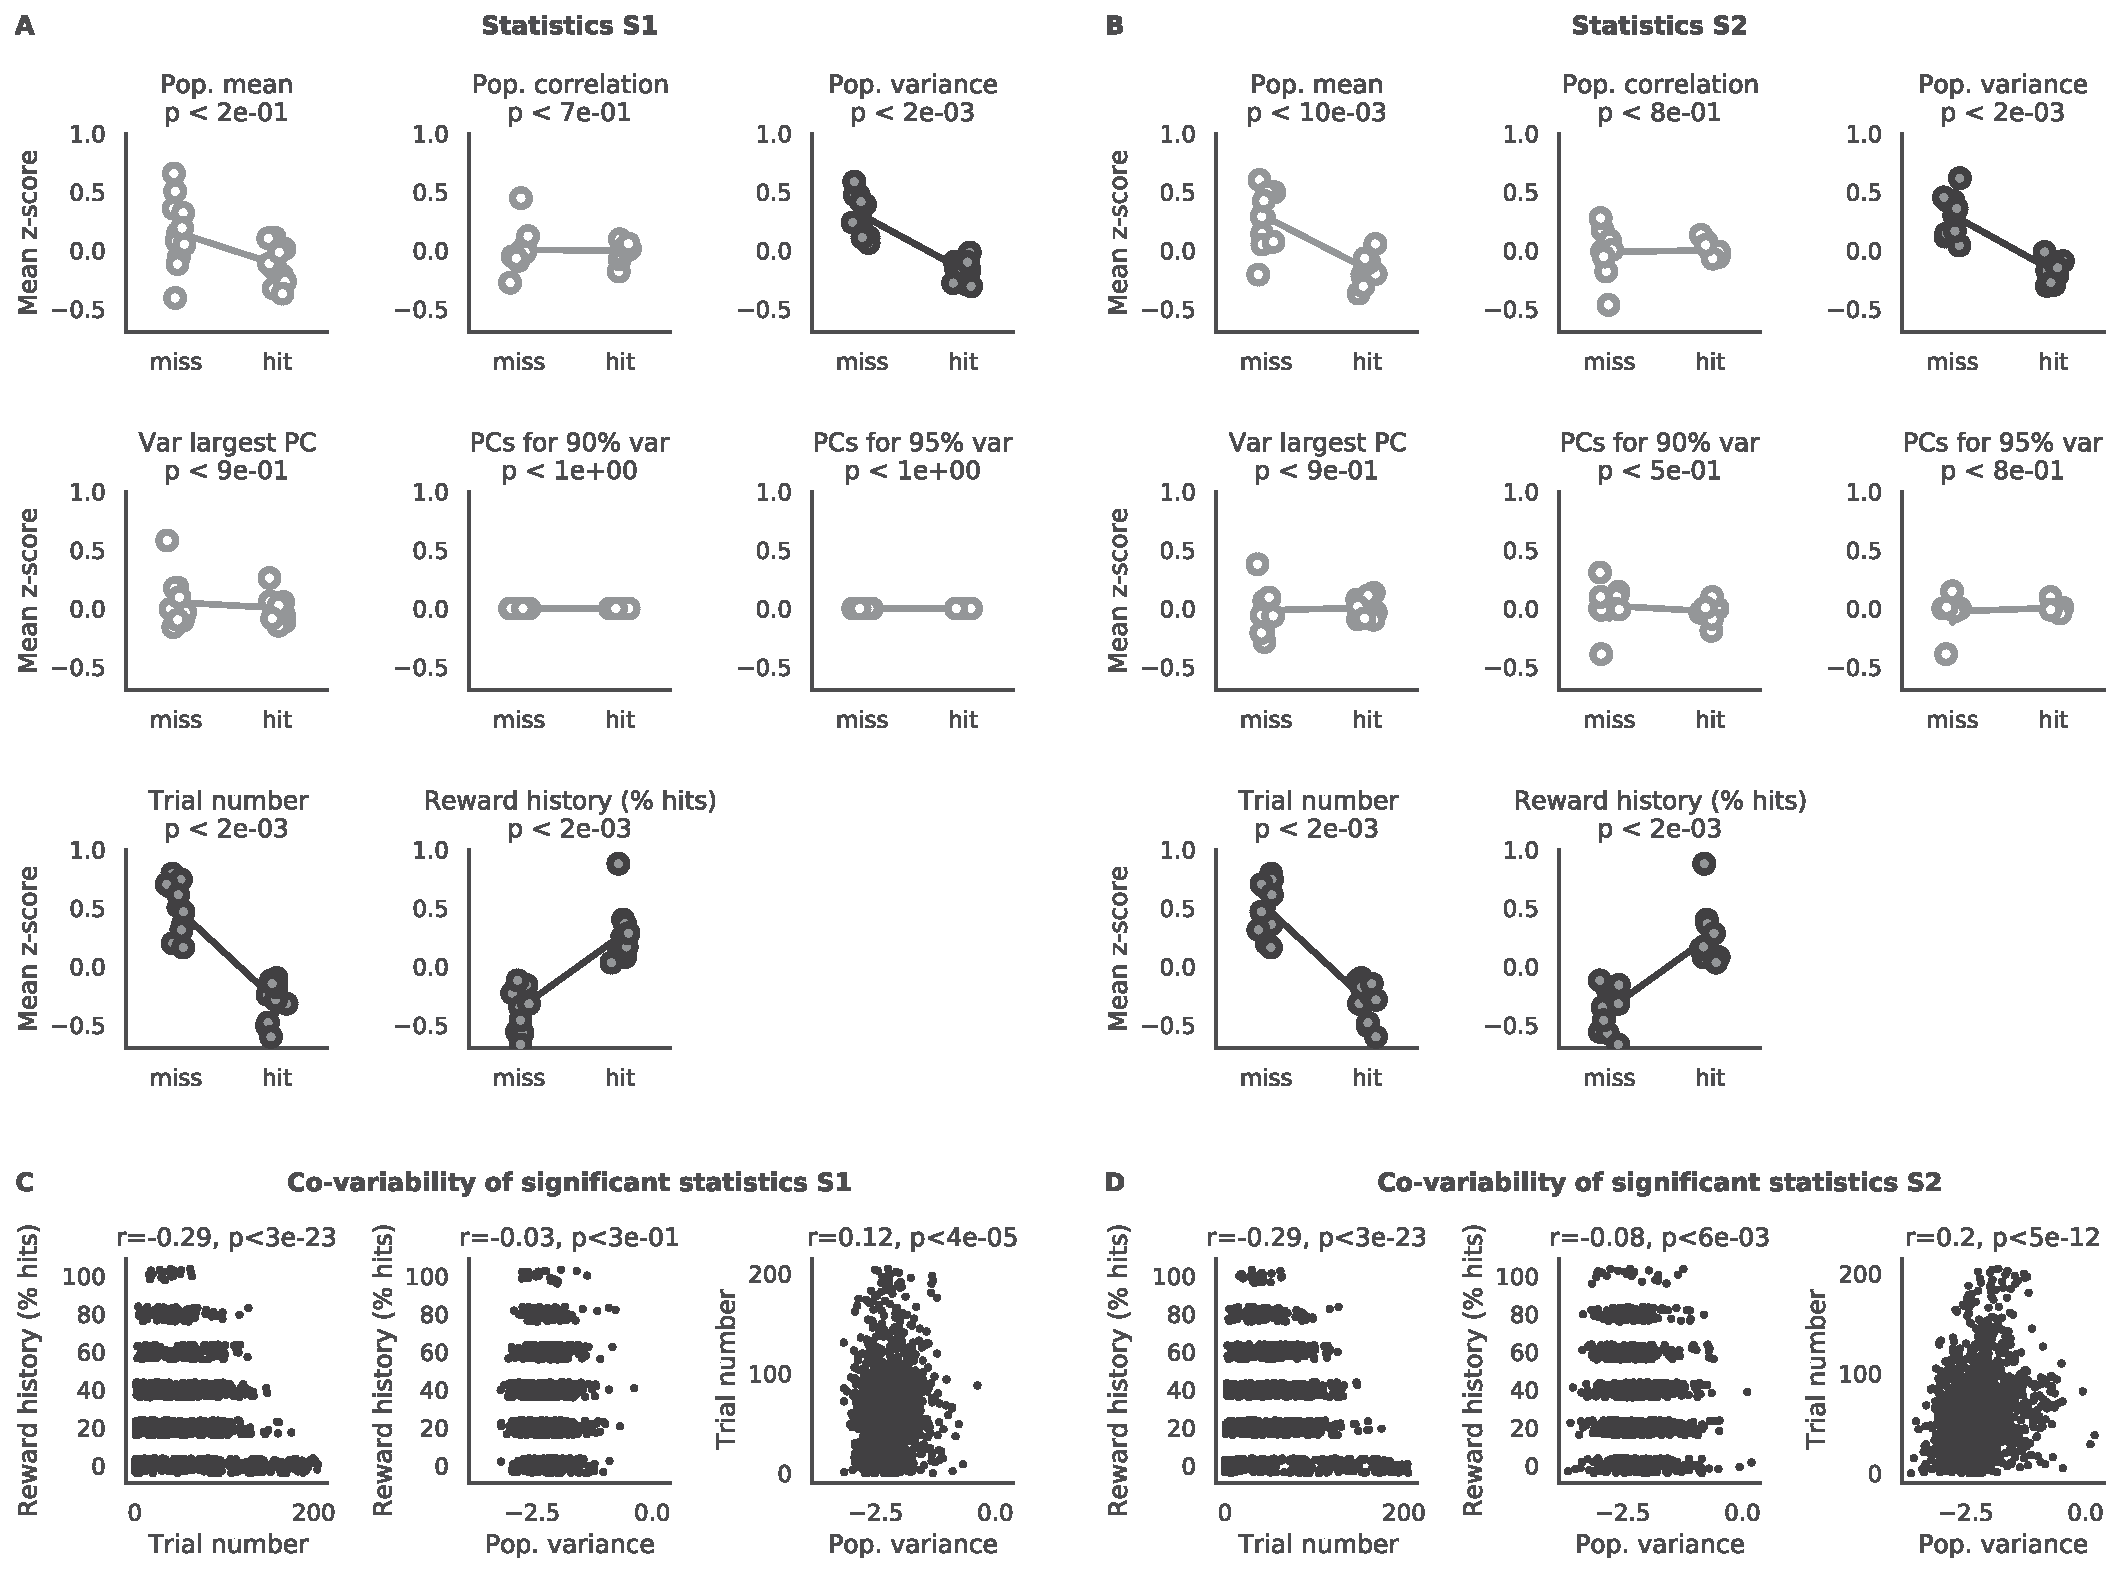
\includegraphics[scale=0.48]{figures/supplements/Supplementary_Figure6.pdf}
\caption[\textbf{Further population metrics of pre-stimulus activity
}]{\textbf{Further population metrics of pre-stimulus activity
} 
Comparison of population metrics of pre-stimulus in  S1 \textbf{(A)} and S2 \textbf{(B)} activity prior to hit trials and prior to miss trials. The top rows show the 3 metrics of Figure 4b. The middle rows show metrics computed using Principal Component Analysis (PCA) \cite{cunningham_dimensionality_2014}: the relative explained variance of the first Principal Components (PC), the number of PCs required for 90\% cumulative explained variance, and the number of PCs required for 95\% explained variance \cite{williamson_scaling_2016}. These are all metrics that indicate how well-structured, or low-dimensional, the covariance matrix is of the neural activity. These metrics are not significant which indicates that the change in population variance is not due a change in covariance structure. The bottom rows show two significant task variables; the trial number (an integer between 0 and the total number of trials in a session, indicating the number of trials previously undertaken by the animal in a given session) and the reward history (defined as \% hit trials in the 5 preceding stimulated trials). \textbf{(C,D)} The co-variability of the significant statistics of panels a and b was assessed using Pearson correlation. Reward history and trial number are strongly correlated, while population variance is significant but weakly correlated to trial number in S1 and both reward history and trial number in S2. 
} 
\label{fig:supp6}
\end{figure}


The relationship between population variance and behavioural performance was also evident on an individual session level, whereby population variance pre-stimulus in S1 is negatively correlated with the probability that the upcoming stimulus elicits a hit (Figure \ref{fig:figure4}D) (one-sided regression test p < 3x10\textsuperscript{-12} on 8/10 sessions, 1 session n.s., 1 session significantly increasing). This result, taken in conjunction with Figure \ref{fig:2-photon-behaviour}G, shows that we have identified two separate conditions that predict the probability that the animal will successfully perceive the stimulus: the strength of the stimulus (number of cells stimulated), and the variance of the population activity (Figure \ref{fig:figure4}B right, D). Next we asked if these two predictors work in tandem, where stimulus perception depends on both the strength of the stimulus and the ongoing state of the population.

We find a clear interaction in which the probability of a stimulus eliciting a hit can be expressed on a two-dimensional axis (Figure \ref{fig:figure4}E), where hit probability is highest when population variance is minimised and the number of cells stimulated is maximised. Stimulating just 5-10 neurons elicited a hit probability of greater than chance level (0.5) when pre-stimulus population variance was at its lowest level, whereas as population variance increased, more stimulated cells were required to reliably drive hits. This phenomenon can be well conceptualised in terms of a signal-to-noise ratio (SNR) framework, in which activity injected into cells through photostimulation forms the signal and the magnitude of background noise is measured as population variance. The higher the SNR, the more likely the animal is to detect the signal above ongoing noise and respond through a hit trial. Indeed, the probability of a hit is highly correlated with SNR when population variance and the number of cells stimulated are collapsed onto an SNR axis (Figure \ref{fig:figure4}F) (p< 2x10\textsuperscript{-10}, logistic regression two-sided t test). Taken together, these results show that the SNR of an incoming stimulus may be critical for its continued propagation out of the local brain region where it was initiated to downstream regions where it can drive behaviour (Figure \ref{fig:figure4}G).